
%(BEGIN_QUESTION)
% Copyright 2010, Tony R. Kuphaldt, released under the Creative Commons Attribution License (v 1.0)
% This means you may do almost anything with this work of mine, so long as you give me proper credit

A computer spreadsheet program may be used as a simulator for an analog-digital converter, taking an analog voltage signal value and converting it into a digital ``count'' value.  

Begin creating your own spreadsheet by following the format shown below, allowing anyone to enter an analog input value in volts, while the spreadsheet calculates the ``count'' value and displays it in decimal, binary, and hexadecimal formats.  Note that the yellow and blue shading in this example spreadsheet is strictly for aesthetic value (distinguishing input values from calculated values) and is not necessary for the spreadsheet to function:

$$\includegraphics[width=15.5cm]{i04408x01.eps}$$

Assume a 0 to 5 volt analog input range, and a 8-bit (00 to FF hex) digital output range.

\vskip 20pt \vbox{\hrule \hbox{\strut \vrule{} {\bf Suggestions for Socratic discussion} \vrule} \hrule}

\begin{itemize}
\item{} How could you modify the spreadsheet to have its analog input range be user-adjustable?  In other words, allowing anyone to simulate the performance of a 0 to 10 volt range or 0 to 20 volt range without having to modify any of the formulae in the spreadsheet?
\item{} How could you {\it test} your spreadsheet cable-length calculator for accuracy (to verify you haven't made any mistakes) once you've entered all your equations?
\end{itemize}

\underbar{file i04408}
%(END_QUESTION)





%(BEGIN_ANSWER)

\begin{itemize}
\item{} Formula for cell {\tt R1C4}: {\tt ROUND((R2C1 / 5) * 255)}
\item{} Formula for cell {\tt R2C4}: {\tt DEC2BIN(R1C4)}
\item{} Formula for cell {\tt R3C4}: {\tt DEC2HEX(R1C4)}
\end{itemize}

%(END_ANSWER)





%(BEGIN_NOTES)


%INDEX% Calibration: table, analog-digital conversion
%INDEX% Computer spreadsheet exercise: analog-digital converter input/output calculations

%(END_NOTES)

